\documentclass{article}
\usepackage{amsfonts}
\usepackage{graphicx}
\usepackage{mathtools}
\title{Assignment 3}
\author{Ernesto Rodriguez}
\begin{document}
\maketitle

\section{Part 1}

\subsection{Problem 1}
If $A \Rightarrow B$, $B$ must be true in every model whare $A$ is true.

By definition $M(A)$ contains all models where $A$ is true. $M(B)$ contains all models where B is true.

This implies all models where $A$ is true must be true for $B$ must be true for $B$ therefore $M(A) \subset M(B)$.

\subsection{Problem 2}

($\Rightarrow$ Proof)

If $\alpha \models \beta$, for all models where $\alpha$ is ture, $\beta$ must be true since $M(\alpha) \subseteq M(\beta)$.

This implies there is no model in $M(\alpha)$ which is false for $\beta$.

($\Leftarrow$ Proof)

If $a \wedge \neg \beta $ is unsatisfiable in any model $M( \alpha )$, $\alpha $ and $\beta $ must be true in all models in $M(  \alpha  )$ since the sentence $ \alpha  \wedge \beta$ must be true for all models in $M( \alpha )$. This means that $\beta$ is true in all models $M( \alpha )$.

\subsection{Problem 3}

($\Rightarrow$ Proof)

If $a$ is valid, then $a$ is true for all models.

The sentence $T$ is also true for all models so: $M(T) \subseteq M( \alpha )$. But since $M(T)$ is all models, the only set which is $M(T)$ is a subset is the same set.

($\Leftarrow$ Proof)

If $M(t) \subseteq M( \alpha )$. T is valid so $M(t)$ is all models. So if $M(T) \subseteq M( \alpha )$, $M( \alpha )$ must also contain all models, so is valid.

\subsection{Problem 4}

If $ \alpha  \models  \beta $ and $ \beta  \models  \alpha $ implies that $M( \alpha ) \subseteq M( \beta )$ and $M( \beta ) \subseteq M( \alpha )$ The only way this is possible if if $M( \alpha )=M( \beta )$ since a set is a subset of itself.

So $ \alpha $ and $ \beta $ are true in the same places of a truth table. By complement they are alos false for the same places as well.

\[
 \alpha  \equiv  \beta  \text{ iff } ( \alpha  \Leftrightarrow  \beta )
\]

($\Rightarrow$ Proof)

$ \alpha  \models  \beta $ and $ \beta  \models  \alpha $ so $M( \alpha )=M( \beta )$. Ths shows that $ \alpha $ and $ \beta $ are true in the same models and there is no model where the value of $ \alpha $ and $ \beta $ can be different.

($\Leftarrow$ Proof)

$ \alpha  \Leftrightarrow  \beta $ if $ \alpha $ imples $ \beta $, every model in $M( \alpha )$ must exist in $M( \beta )$; $M( \alpha ) \subseteq M( \beta )$. Likewise if $ \beta $ implies $ \alpha $ all models $M( \beta )$ must exist in $M( \alpha )$; $M( \beta ) \subseteq M( \alpha )$.

This imples $M( \alpha )=M( \beta )$ and this implies that the TT of $ \alpha $ and $ \beta $ are the same.

\subsection{Problem 5}

The truth table for the sentence $(( \alpha  \Rightarrow  \beta ) \wedge  \alpha ) \models  \beta $:

\begin{tabular}{ | c | c | c | c | }

\hline
{\bf $ \alpha $} & {\bf $ \beta $} & {\bf $ \alpha  \Rightarrow  \beta $} & {\bf $(( \alpha  \Rightarrow  \beta ) \wedge  \alpha ) \models  \beta $} \\
\hline
T & T & T & T \\
\hline
T & F & T & F \\
\hline
F & T & F & F \\
\hline
F & F & T & F\\
\hline
\end{tabular}

As we can see, when $(( \alpha  \Rightarrow  \beta ) \wedge  \alpha )$ is true, $ \beta $ is also true.

\subsection{Problem 6}

\begin{tabular}{ | c | c | c | }
\hline
{\bf $ \alpha $} & {\bf $ \beta $} & {\bf $ \alpha \wedge  \beta $} \\
T & T & T \\
\hline
T & F & F \\
\hline
F & T & F \\
\hline
F & F & F \\
\hline
\end{tabular}

\subsection{Problem 7}

Proove that:

\[
(S_1 \vee S_2 \vee ... \vee S_k) \wedge (\neg S_i) \models S_i \vee ... \vee S_{i-1} \vee S_{i+1} \vee ... \vee S_k 
\]

Lets firt consider the sentence on the left:

\[
(S_1 \vee S_2 \vee ... \vee S_k) \wedge (\neg S_i)
\]

For it to be true, $S_i$ must be false since it's presented as a and at the end of the sentence. So we can rewrite:

\[
(S_i \vee ... \vee S_{i-1} \vee False \vee S_{i+i} \vee ... S_k) \wedge True
\]

Which translates to:

\[
(S_i \vee ... \vee S_{i-1} \vee S_{i+i} \vee ... S_k)
\]

\subsection{Problem 8}

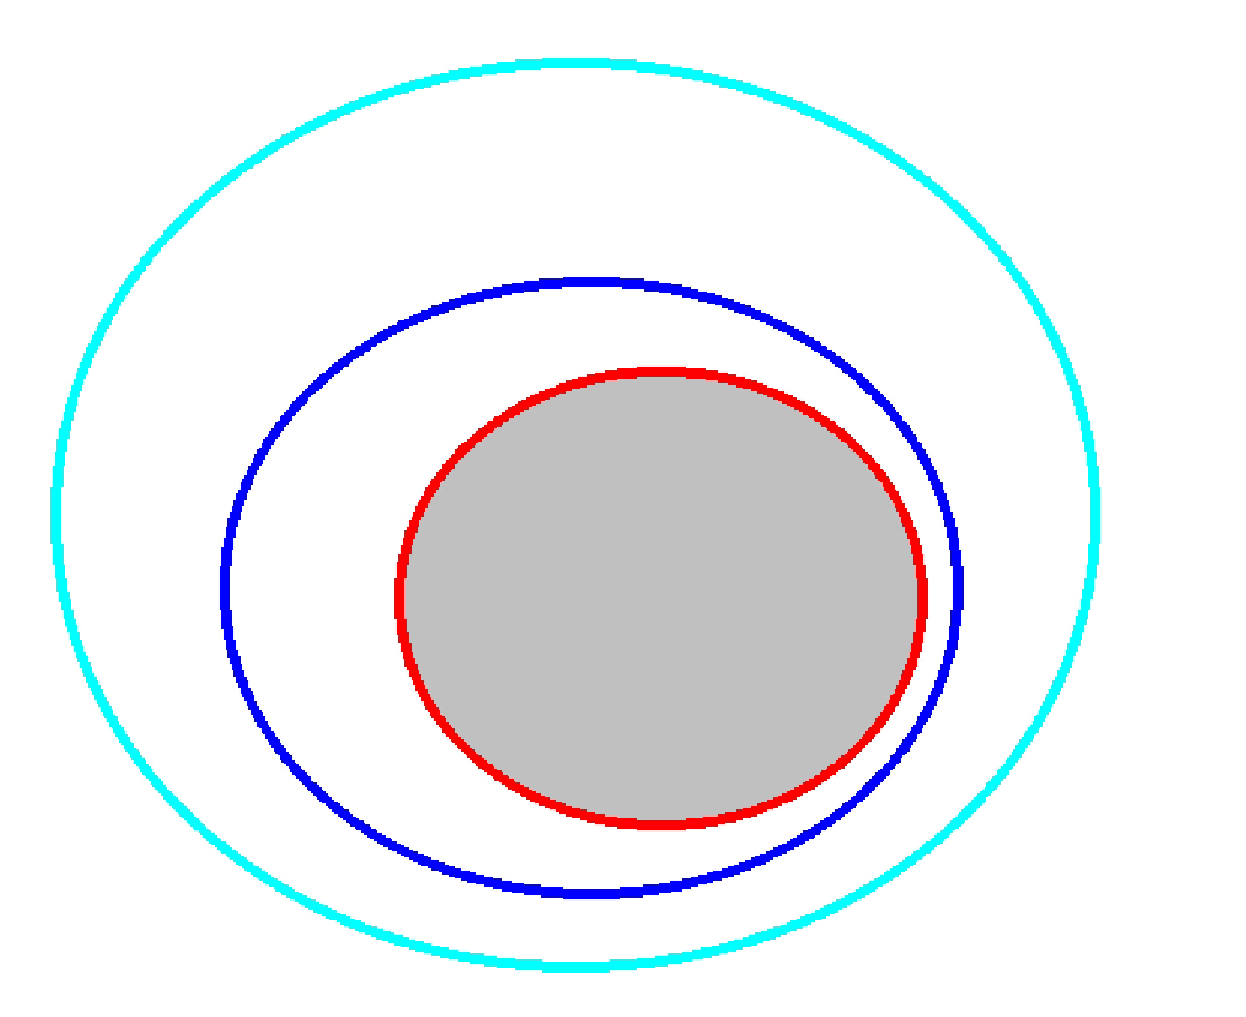
\includegraphics[width=100mm]{entails.eps}

The cyan represents $M(C)$ the blue represents $M(B)$ and the red represents $M(A)$. The gray area is $(A \models B) \wedge (B \models C)$. As we can se it is a subset of $M(C)$.

\subsection{Problem 9}

TT for the sentence $(\neg A \vee X) \wedge (A \vee Y) \models (X \vee Y)$:

\begin{tabular}{ | c | c | c | c | c | c | c | c | }
\hline
{\bf $A$} & {\bf $X$} & {\bf $Y$} & {\bf $\neg A$} & {\bf $\neg A \vee X$} & {\bf $A \vee Y$} & {\bf $(\neg A \vee X) \wedge (A \vee Y)$} & {\bf $(X \vee Y)$} \\
\hline
T & T & T & F & T & T & T & T \\
\hline
T & T & F & F & T & T & T & T \\
\hline
T & F & T & F & F & T & F & T \\
\hline
T & F & F & F & F & T & F & F \\
\hline
F & T & T & T & T & T & T & T \\
\hline
F & T & F & T & T & F & F & T \\
\hline
F & F & T & T & T & T & T & T \\
\hline
F & F & F & T & T & F & F & F \\
\hline
\end{tabular}

\section{Part 2}

\begin{itemize}

\item{{\bf $A \Leftrightarrow (C \vee E)$:} 

  $\rightarrow$ $(\neg A \vee (C \vee E)) \wedge (\neg (C \vee E) \vee A)$

  $\rightarrow$ $(\neg A \vee C \vee E) \wedge (\neg A \wedge \neg E \vee A)$
  
  $\rightarrow$ $(\neg A \vee C \vee E) \wedge (\neg A \vee A) \wedge (\neg B \vee A)$

  $\rightarrow$ $(\neg A \vee C \vee E) \wedge (\neg B \vee A)$}

\item{{\bf $E \Rightarrow D$:}

  $(E \wedge D) \vee \neg D$

  $(E \vee \neg D) \wedge (D \vee \neg D)$

  $(E \vee \neg D)$}

\item{{\bf $B \wedge F \Rightarrow \neg C$}:
    
  $((B \wedge F) \wedge \neg C) \vee C$

  $(B \vee C) \wedge (F \vee C) \wedge (C \vee \neg C)$

  $(B \vee C) \wedge (F \vee C)$}

\item{{\bf $E \Rightarrow C$:}

  $(E \vee \neg C)$}

\item{{\bf $C \Rightarrow F$:}

  $(C \vee \neg F)$}

\item{{\bf $C \Rightarrow B$:}

  $(C \vee \neg B)$}

\end{itemize}


{\bf DPLL Trace for the clauses: $(\neg A \vee C \vee E),(\neg B \vee A),(E \vee \neg D),(B \vee C),(F \vee C),(E \vee \neg C),(C \vee \neg F),(C \vee \neg B)$}

\begin{tabular}{|c|c|c|c|}

\hline
{\bf Iteration} & {\bf Symbols} & {\bf Model} & {\bf Action} \\
\hline
1 & a,b,c,d,e & & pure symbol e=T \\
\hline
2 & a,b,c,d & e=T & Try a=T \\
\hline
3 & b,c,d & a=T,e=T & Try b=T \\
\hline
4 & c,d & a=T,b=T,e=T & Found unit clause: $(c \vee \neg b)$. Set c=T \\
\hline
5 & d & a=T,b=T,c=T,e=T & All clauses are true, return T \\
\hline
\end{tabular}

\end{document}

